\documentclass[12pt,letterpaper, oneside]{book}
\usepackage{tabularx}
\usepackage{longtable}
\usepackage[utf8]{inputenc}
\usepackage[T1]{fontenc}
\usepackage{changepage}
\usepackage{mathptmx} % times font
\usepackage[spanish,es-tabla, es-lcroman]{babel}
\usepackage{amsmath}
\usepackage{amsfonts}
\usepackage{amssymb}
\usepackage{listings}
\usepackage{graphicx}
\usepackage[document]{ragged2e}
\usepackage{subfig}
\usepackage{wasysym}
\usepackage{lscape}
\usepackage[colorlinks=true, linkcolor=black,
citecolor=black, urlcolor=black,hidelinks]{hyperref}
\usepackage{float}
\usepackage{booktabs}
\usepackage{setspace}
\usepackage{xcolor}
\usepackage{lipsum}
\usepackage[left=4cm,top=4cm,right=2.6cm,,bottom=2.6cm]{geometry}
\usepackage[justification=centering]{caption}
\usepackage{hyperref}
\usepackage{adjustbox}



\captionsetup{belowskip=0pt}

\newcommand{\grad}{$^{\circ}$}
\renewcommand{\baselinestretch}{1.5}

\usepackage[authoryear,round,sort]{natbib}

\renewcommand{\labelenumii}{\arabic{enumi}.\arabic{enumii}}
\renewcommand{\labelenumiii}{\arabic{enumi}.\arabic{enumii}.\arabic{enumiii}}
\renewcommand{\labelenumiv}{\arabic{enumi}.\arabic{enumii}.\arabic{enumiii}.\arabic{enumiv}}
\renewcommand{\chaptername}{}

\definecolor{codegreen}{rgb}{0,0.6,0}
\definecolor{codegray}{rgb}{0.5,0.5,0.5}
\definecolor{codepurple}{rgb}{0.58,0,0.82}
\definecolor{backcolour}{rgb}{0.95,0.95,0.92}

\lstdefinestyle{mystyle}{
    backgroundcolor=\color{backcolour},
    commentstyle=\color{codegreen},
    keywordstyle=\color{magenta},
    numberstyle=\tiny\color{codegray},
    stringstyle=\color{codepurple},
    basicstyle=\ttfamily\footnotesize,
    breakatwhitespace=false,
    breaklines=true,
    captionpos=b,
    keepspaces=true,
    numbers=left,
    numbersep=5pt,
    showspaces=false,
    showstringspaces=false,
    showtabs=false,
    tabsize=2
}
\lstset{style=mystyle}


\usepackage{titlesec}

\titleformat{\chapter}
  {\normalfont\normalsize\bfseries}{\thechapter}{0.5em}{}

\titleformat{\section}
  {\normalfont\normalsize\bfseries}{\thesection.}{0.5em}{}
\titleformat{\subsection}
  {\normalfont\normalsize\bfseries}{\thesubsection.}{0.5em}{}

\usepackage{fancyhdr}
\fancyhf{}
\renewcommand\headrulewidth{0pt}
\fancyfoot[R]{\thepage}
\pagestyle{fancy}
\fancypagestyle{plain}{%
    \renewcommand{\headrulewidth}{0pt}%
    \fancyhf{}%
    \fancyfoot[R]{\thepage}%
}

\usepackage[subfigure]{tocloft}
\setlength{\cftsecindent}{0em}
\setlength{\cftsubsecindent}{0em}
\setlength{\cftsubsubsecindent}{0em}

\usepackage{enumitem}
\setcounter{tocdepth}{4}
\setcounter{secnumdepth}{4}

\makeatletter
\patchcmd{\chapter}{\if@openright\cleardoublepage\else\clearpage\fi}{}{}{}
\makeatother

\usepackage{chngcntr}
\counterwithout{figure}{chapter}

\addto\captionsspanish{%
  \renewcommand{\contentsname}%
    {\fontsize{16}{20}\selectfont ÍNDICE}
}

\setlength{\cftbeforetoctitleskip}{-1em}
\setlength{\cftaftertoctitleskip}{1em}

\setlength\parindent{0pt}

\setlength{\parskip}{0.5em}
\unaccentedoperators

\begin{document}
	%FRONTMATTER
	%---------------------------------------------------
	\frontmatter
	\newgeometry{top=2.5cm, bottom=2.5cm, left=2.5cm, right=2.5cm}
    \begin{titlepage}
	\begin{center}
	    {\fontsize{20}{20}\selectfont \textbf{UNIVERSIDAD MAYOR DE SAN ANDRÉS}}\\
		{\fontsize{16}{16}\selectfont \textbf{FACULTAD DE CIENCIAS PURAS Y NATURALES\\
		CARRERA DE INFORMÁTICA}}

		
\includegraphics[scale=0.20]{logo_umsa.png}

		{\fontsize{16}{20}\selectfont \textbf{TRABAJO DE INVESTIGACIÓN}}\\

        {\fontsize{16}{18}\selectfont \textbf{DETECCIÓN DE ANOMALÍAS EN LOGS DE UN SISTEMA DE REPORTES DE VENTAS MEDIANTE ALGORITMOS DE MINERÍA DE DATOS}}

		{\fontsize{12}{12}\selectfont\textbf{Trabajo de Investigación para la Materia de Minería de Datos}}

		{\fontsize{16}{16}\selectfont\textbf{POR: ROLANDO TROCHE VENEGAS}}\\
    	{\fontsize{14}{14}\selectfont\textbf{}}

		\textbf{LA PAZ - BOLIVIA\\
		2026}
	\end{center}
\end{titlepage}
\restoregeometry

	\tableofcontents
	\setcounter{page}{1}

	\mainmatter

    \raggedbottom

    \thispagestyle{empty}

    % =========================================================
    \chapter{INTRODUCCIÓN}
    % =========================================================

    En los sistemas de software modernos, los registros de eventos o \textit{logs}
    constituyen una fuente fundamental de información operativa. Cada solicitud que
    un usuario realiza queda trazada a través de múltiples capas de servicios,
    generando miles de entradas por minuto que describen el comportamiento del
    sistema en tiempo real. La capacidad de analizar estos registros de manera
    eficiente determina en gran medida la velocidad con la que un equipo de
    operaciones puede detectar, diagnosticar y resolver incidentes \citep{he2016experience}.

    La detección de anomalías en logs es el proceso de identificar patrones de
    comportamiento que se desvían significativamente de lo esperado, ya sea por
    degradación del rendimiento, errores en cascada, uso excesivo de recursos o
    exportaciones de datos inusualmente grandes \citep{chandola2009anomaly}. En
    entornos distribuidos, donde una sola transacción de usuario atraviesa varios
    microservicios, estas anomalías pueden propagarse silenciosamente hasta
    convertirse en fallos críticos si no se detectan a tiempo \citep{xu2009detecting}.

    El presente trabajo aplica técnicas de minería de datos no supervisadas
    —\textit{Isolation Forest}, \textit{Local Outlier Factor} y \textit{One-Class SVM}—
    sobre registros de un sistema de reportes de ventas compuesto por tres capas de
    servicio: \textit{Report Service}, \textit{Sales API} y base de datos. El conjunto
    de datos contiene 30\,000 registros de logs correspondientes al mes de enero de
    2026, de los cuales el 4,55\% corresponde a anomalías de cuatro tipos distintos:
    consultas lentas a la base de datos, exportaciones de reportes de gran tamaño,
    alta tasa de errores y uso excesivo de recursos computacionales.

    El trabajo se organiza de la siguiente manera: el Capítulo~2 diagnostica la
    problemática del monitoreo manual de logs; el Capítulo~3 establece los objetivos
    de la investigación; el Capítulo~4 describe el proceso de análisis de datos,
    incluyendo la fuente, preparación y modelado; el Capítulo~5 presenta los
    resultados comparativos de los tres modelos; y el Capítulo~6 expone las
    conclusiones derivadas del estudio.

    % =========================================================
    \chapter{DIAGNÓSTICO Y PLANTEAMIENTO DEL PROBLEMA}
    % =========================================================

    \section{PLANTEAMIENTO DEL PROBLEMA}

    Los sistemas empresariales de reportes de ventas procesan continuamente
    solicitudes de múltiples usuarios con distintos roles —administradores,
    gerentes y vendedores— para generar informes de diversa complejidad:
    ventas diarias, mensuales, por producto, por sucursal y por cliente.
    Estas operaciones involucran una cadena de servicios que puede describirse
    de la siguiente manera:

    \begin{center}
    \textbf{Usuario} $\rightarrow$ \textbf{Report Service} $\rightarrow$
    \textbf{Sales API} $\rightarrow$ \textbf{Base de Datos}
    \end{center}

    Cada capa registra métricas de rendimiento propias, incluyendo tiempos de
    respuesta, cantidad de registros procesados, uso de CPU y memoria, códigos
    de estado HTTP, conteo de errores y número de reintentos. Bajo condiciones
    normales de operación, estas métricas se mantienen dentro de rangos esperados
    que varían según el tipo de reporte solicitado.

    El problema central radica en la \textbf{detección oportuna de comportamientos
    anómalos} dentro de este flujo de datos. Cuatro categorías de anomalías
    afectan con mayor frecuencia a este tipo de sistemas:

    \begin{enumerate}
        \item \textbf{Consultas lentas a la base de datos} (\textit{slow\_database\_query}):
        el tiempo de consulta se multiplica entre 8 y 20 veces respecto al valor
        esperado, con un aumento proporcional en las filas escaneadas. Esta
        anomalía suele indicar ausencia de índices adecuados, bloqueos de tabla
        o degradación del motor de base de datos.

        \item \textbf{Exportaciones de reportes de gran tamaño} (\textit{large\_report\_export}):
        la cantidad de registros retornados y el tamaño del reporte se incrementan
        entre 10 y 50 veces, provocando una presión excesiva sobre la memoria del
        servicio. Este patrón puede indicar filtros mal configurados o solicitudes
        maliciosas de extracción masiva de datos.

        \item \textbf{Alta tasa de errores} (\textit{high\_error\_rate}): los
        códigos de estado HTTP cambian a valores 5xx (500, 502, 503, 504), con
        múltiples reintentos por solicitud. Señala inestabilidad en el servicio
        o en la conectividad entre capas.

        \item \textbf{Alto uso de recursos} (\textit{high\_resource\_usage}):
        el uso de CPU supera el 85\% y el consumo de memoria se multiplica entre
        3 y 7 veces, degradando la disponibilidad del servicio para otros usuarios.
    \end{enumerate}

    El monitoreo manual de estos patrones resulta inviable a escala: un sistema
    con 120 usuarios activos y 10\,000 solicitudes mensuales genera 30\,000
    entradas de log distribuidas en tres servicios. La revisión humana no puede
    operar en tiempo real, lo que genera una brecha entre la ocurrencia de una
    anomalía y su detección. La aplicación de algoritmos de minería de datos
    ofrece una solución escalable para automatizar este proceso de vigilancia
    \citep{zhang2019robust}.

    % =========================================================
    \chapter{OBJETIVO DE LA INVESTIGACIÓN}
    % =========================================================

    \section{OBJETIVO GENERAL}

    Aplicar y comparar algoritmos de detección de anomalías no supervisados
    (\textit{Isolation Forest}, \textit{Local Outlier Factor} y \textit{One-Class SVM})
    sobre los registros de logs de un sistema de reportes de ventas distribuido,
    con el fin de identificar automáticamente comportamientos anómalos en el
    flujo Usuario $\rightarrow$ Report Service $\rightarrow$ Sales API $\rightarrow$
    Base de Datos.

    \section{OBJETIVOS ESPECÍFICOS}

    \begin{enumerate}
        \item Realizar un análisis exploratorio de los datos de logs del sistema
        de reportes de ventas, identificando la distribución de las variables
        numéricas, la prevalencia de cada tipo de anomalía y los patrones
        temporales de ocurrencia.

        \item Preprocesar el conjunto de datos mediante codificación de variables
        categóricas y normalización de características numéricas para su uso como
        entrada en modelos de aprendizaje automático.

        \item Implementar y entrenar tres modelos de detección de anomalías
        no supervisados: \textit{Isolation Forest}, \textit{Local Outlier Factor}
        con novedad y \textit{One-Class SVM}, entrenados exclusivamente con
        registros normales.

        \item Evaluar y comparar el desempeño de los tres modelos utilizando
        las métricas de precisión, \textit{recall}, F1-Score y AUC-ROC,
        contrastando las predicciones contra las etiquetas de verdad absoluta
        disponibles en el conjunto de datos.

        \item Determinar las variables con mayor poder discriminativo para la
        detección de anomalías mediante análisis de importancia de características
        sobre el modelo de \textit{Isolation Forest}.
    \end{enumerate}

    % =========================================================
    \chapter{ANÁLISIS DE LA INFORMACIÓN}
    % =========================================================

    \section{FUENTE DE DATOS}

    El conjunto de datos utilizado en este estudio fue generado sintéticamente
    mediante un script de Python que simula el flujo de logs real de un sistema
    de reportes de ventas empresarial. Esta aproximación permite contar con
    etiquetas de verdad absoluta (\textit{ground truth}) para la evaluación
    rigurosa de los modelos, siguiendo la metodología de \citet{du2017deeplog}
    para la generación controlada de anomalías en logs.

    El conjunto de datos contiene \textbf{30\,000 registros}, distribuidos
    uniformemente entre tres servicios:

    \begin{itemize}
        \item \textbf{Report Service}: 10\,000 registros (punto de entrada del usuario).
        \item \textbf{Sales API}: 10\,000 registros (capa intermedia de lógica de negocio).
        \item \textbf{Base de Datos}: 10\,000 registros (capa de persistencia).
    \end{itemize}

    Los registros corresponden a \textbf{10\,000 trazas únicas} (\textit{trace\_id}),
    cada una representando una solicitud completa de reporte desde el usuario hasta
    la base de datos, durante el período del 1 al 31 de enero de 2026. El sistema
    cuenta con 120 usuarios únicos distribuidos en 20 tenants, con roles de
    administrador, gerente y vendedor.

    Cada registro incluye las siguientes variables:

    \begin{longtable}{lp{8cm}}
    \toprule
    \textbf{Variable} & \textbf{Descripción} \\
    \midrule
    \endfirsthead
    \toprule
    \textbf{Variable} & \textbf{Descripción} \\
    \midrule
    \endhead
    \texttt{timestamp} & Marca temporal del evento (ISO 8601) \\
    \texttt{trace\_id} & Identificador único de la traza de solicitud \\
    \texttt{service} & Servicio que generó el log \\
    \texttt{user\_hash} & Identificador anonimizado del usuario \\
    \texttt{tenant\_hash} & Identificador anonimizado del tenant \\
    \texttt{user\_role} & Rol del usuario (admin, manager, seller) \\
    \texttt{report\_type} & Tipo de reporte solicitado \\
    \texttt{status\_code} & Código de estado HTTP de la respuesta \\
    \texttt{response\_time\_ms} & Tiempo de respuesta total del servicio (ms) \\
    \texttt{db\_query\_time\_ms} & Tiempo de consulta a la base de datos (ms) \\
    \texttt{api\_response\_time\_ms} & Tiempo de respuesta de la Sales API (ms) \\
    \texttt{records\_returned} & Número de registros retornados \\
    \texttt{rows\_scanned} & Número de filas escaneadas en la DB \\
    \texttt{report\_size\_kb} & Tamaño del reporte generado (KB) \\
    \texttt{cpu\_usage\_percent} & Uso de CPU del servicio (\%) \\
    \texttt{memory\_usage\_mb} & Uso de memoria RAM (MB) \\
    \texttt{retry\_count} & Número de reintentos de la solicitud \\
    \texttt{error\_count} & Número de errores registrados \\
    \texttt{is\_anomaly} & Etiqueta binaria (0=normal, 1=anomalía) \\
    \texttt{anomaly\_type} & Tipo específico de anomalía o "normal" \\
    \bottomrule
    \caption{Variables del conjunto de datos de logs.}
    \label{tab:variables}
    \end{longtable}

    La distribución de anomalías en el conjunto de datos es la siguiente:

    \begin{table}[H]
    \centering
    \begin{tabular}{lrr}
    \toprule
    \textbf{Tipo de anomalía} & \textbf{Cantidad} & \textbf{Porcentaje} \\
    \midrule
    Normal & 28\,635 & 95,45\% \\
    Consulta lenta a DB (\textit{slow\_database\_query}) & 399 & 1,33\% \\
    Alto uso de recursos (\textit{high\_resource\_usage}) & 339 & 1,13\% \\
    Exportación grande (\textit{large\_report\_export}) & 315 & 1,05\% \\
    Alta tasa de errores (\textit{high\_error\_rate}) & 312 & 1,04\% \\
    \midrule
    \textbf{Total} & \textbf{30\,000} & \textbf{100\%} \\
    \bottomrule
    \end{tabular}
    \caption{Distribución de tipos de anomalía en el conjunto de datos.}
    \label{tab:anomaly_dist}
    \end{table}

    \section{PREPARACIÓN DE LOS DATOS}

    \subsection{Exploración y Análisis Descriptivo}

    El análisis exploratorio inicial se centró en el servicio \textit{report-service},
    por ser el punto de entrada de las solicitudes y el que acumula los efectos de
    anomalías en las capas inferiores. Las estadísticas descriptivas de las
    principales variables numéricas son las siguientes:

    \begin{table}[H]
    \centering
    \begin{tabular}{lrrrrr}
    \toprule
    \textbf{Variable} & \textbf{Media} & \textbf{Desv. Est.} & \textbf{Mín.} & \textbf{Med.} & \textbf{Máx.} \\
    \midrule
    T. respuesta (ms) & 3\,995,77 & 5\,021,09 & 933 & 3\,084 & 96\,135 \\
    T. consulta DB (ms) & 1\,429,42 & 2\,236,65 & 128 & 1\,074 & 60\,700 \\
    Registros retornados & 5\,820,12 & 15\,222,27 & 100 & 3\,990 & 424\,502 \\
    CPU (\%) & 43,21 & 13,96 & 20,00 & 42,91 & 98,91 \\
    Memoria (MB) & 782,54 & 537,64 & 250 & 738 & 8\,330 \\
    \bottomrule
    \end{tabular}
    \caption{Estadísticas descriptivas del servicio \textit{report-service}.}
    \label{tab:estadisticas}
    \end{table}

    La alta desviación estándar en variables como el tiempo de respuesta
    (5\,021 ms frente a una media de 3\,995 ms) y los registros retornados
    (15\,222 frente a una media de 5\,820) evidencia la presencia de valores
    extremos introducidos por las anomalías. El valor máximo del tiempo de
    respuesta (96\,135 ms) corresponde a anomalías de consulta lenta, mientras
    que el máximo de registros retornados (424\,502) corresponde a exportaciones
    de gran tamaño.

    La Figura~\ref{fig:anomaly_dist} muestra la distribución de los tipos de
    anomalía tanto de manera global como por servicio.

    \begin{figure}[H]
    \centering
    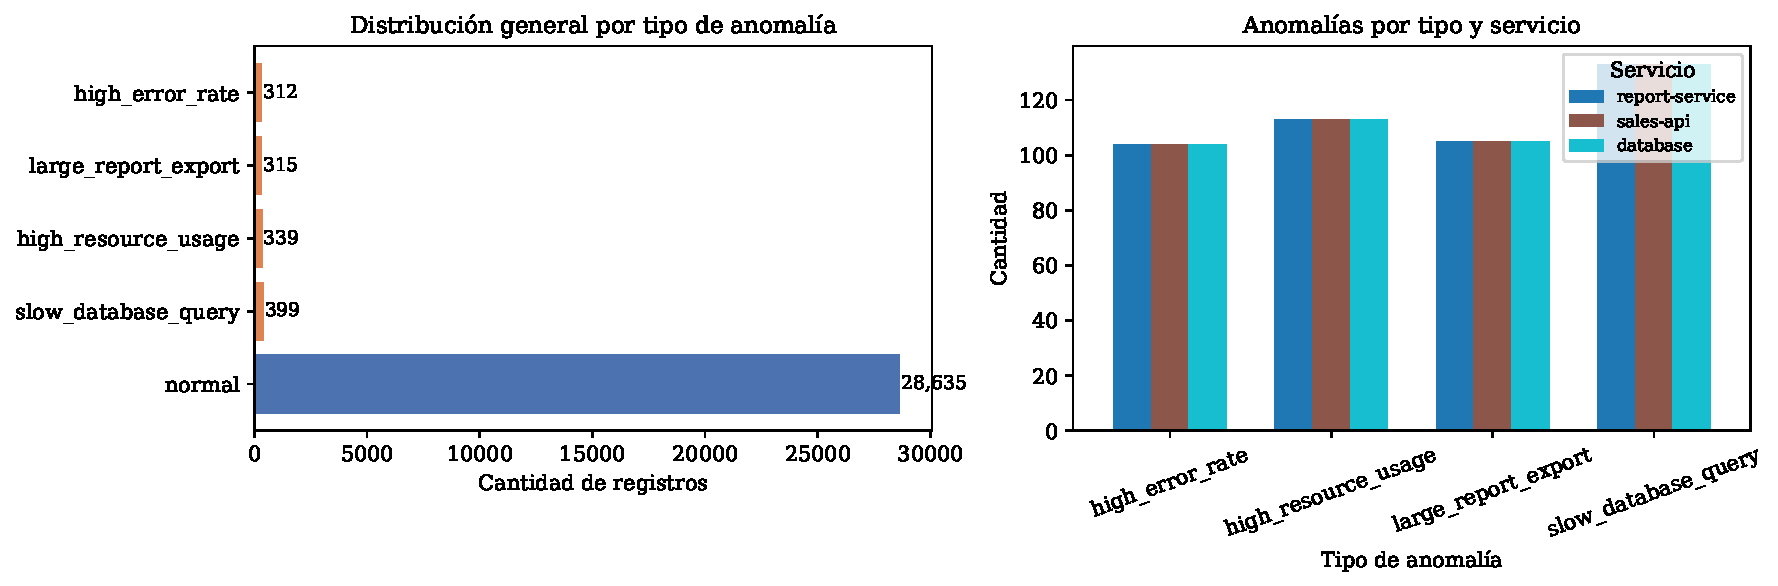
\includegraphics[width=\textwidth]{figures/fig_anomaly_distribution.pdf}
    \caption{Distribución de tipos de anomalía: global (izquierda) y por servicio (derecha).}
    \label{fig:anomaly_dist}
    \end{figure}

    Se observa que la distribución de anomalías es uniforme entre los tres
    servicios, lo cual es esperable dado que cada anomalía se propaga a través
    de toda la cadena de servicios dentro de la misma traza. Las consultas
    lentas a la base de datos son ligeramente más frecuentes (399 instancias),
    seguidas por el alto uso de recursos (339), exportaciones grandes (315)
    y alta tasa de errores (312).

    La Figura~\ref{fig:response_time} presenta los diagramas de caja del tiempo
    de respuesta y del tiempo de consulta a la base de datos, segmentados por
    tipo de anomalía.

    \begin{figure}[H]
    \centering
    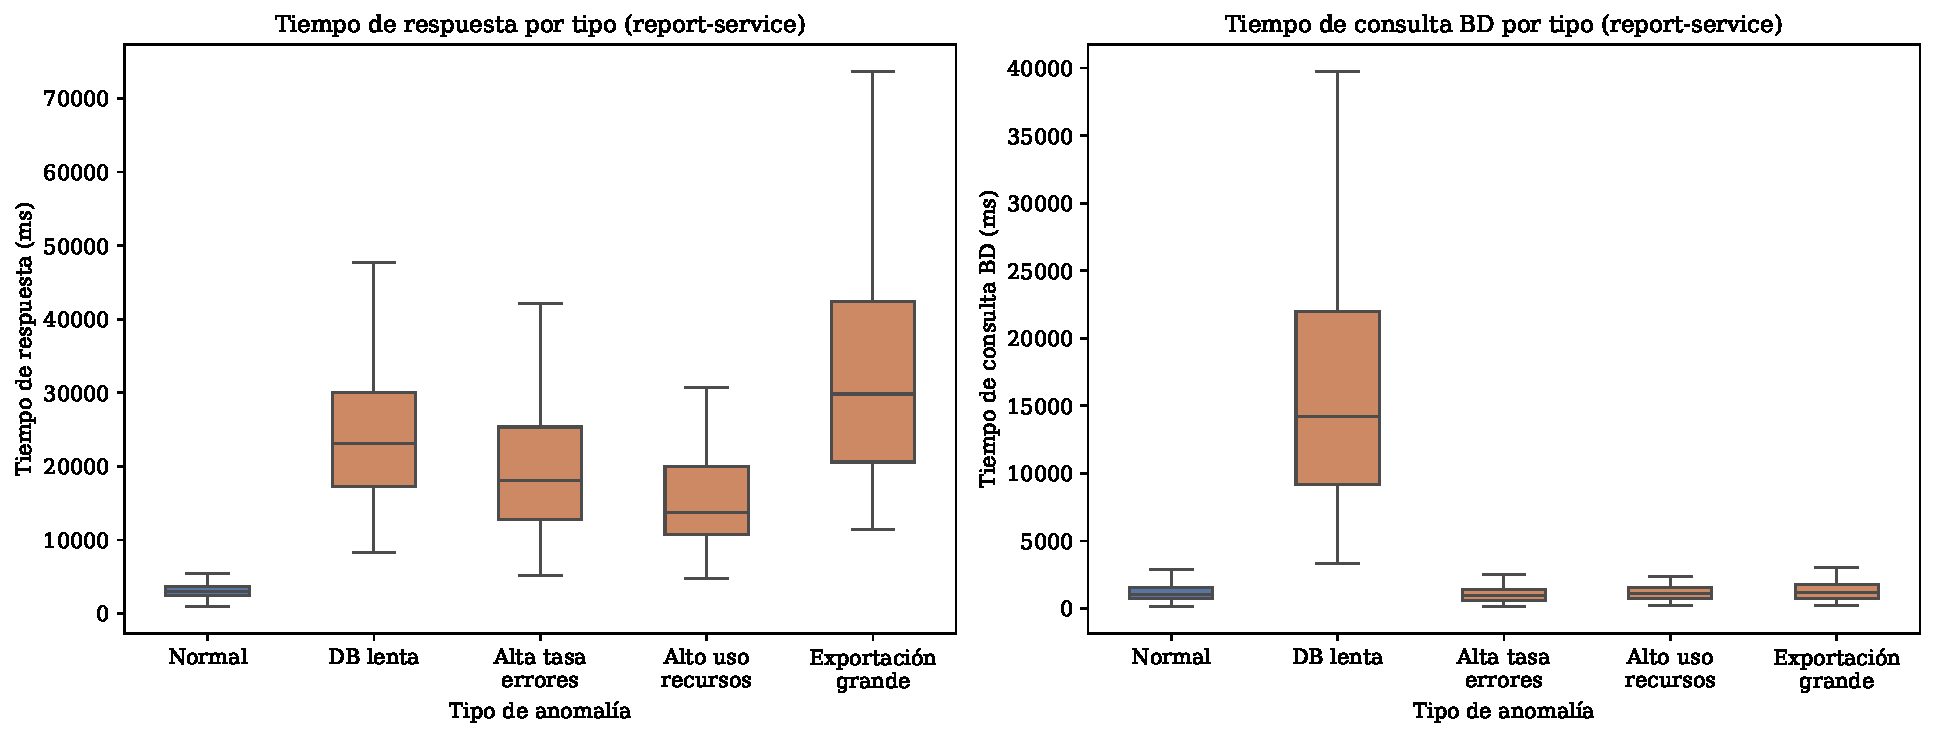
\includegraphics[width=\textwidth]{figures/fig_response_time_boxplot.pdf}
    \caption{Distribución de tiempos de respuesta por tipo de anomalía en \textit{report-service}.}
    \label{fig:response_time}
    \end{figure}

    La figura confirma que las anomalías de consulta lenta a la base de datos
    producen los tiempos de respuesta más elevados, seguidas por las exportaciones
    de gran tamaño. Las anomalías de alta tasa de errores y alto uso de recursos
    también muestran tiempos de respuesta significativamente superiores al caso
    normal, aunque con menor magnitud.

    La Figura~\ref{fig:correlation} presenta la matriz de correlación entre las
    variables numéricas del conjunto de datos.

    \begin{figure}[H]
    \centering
    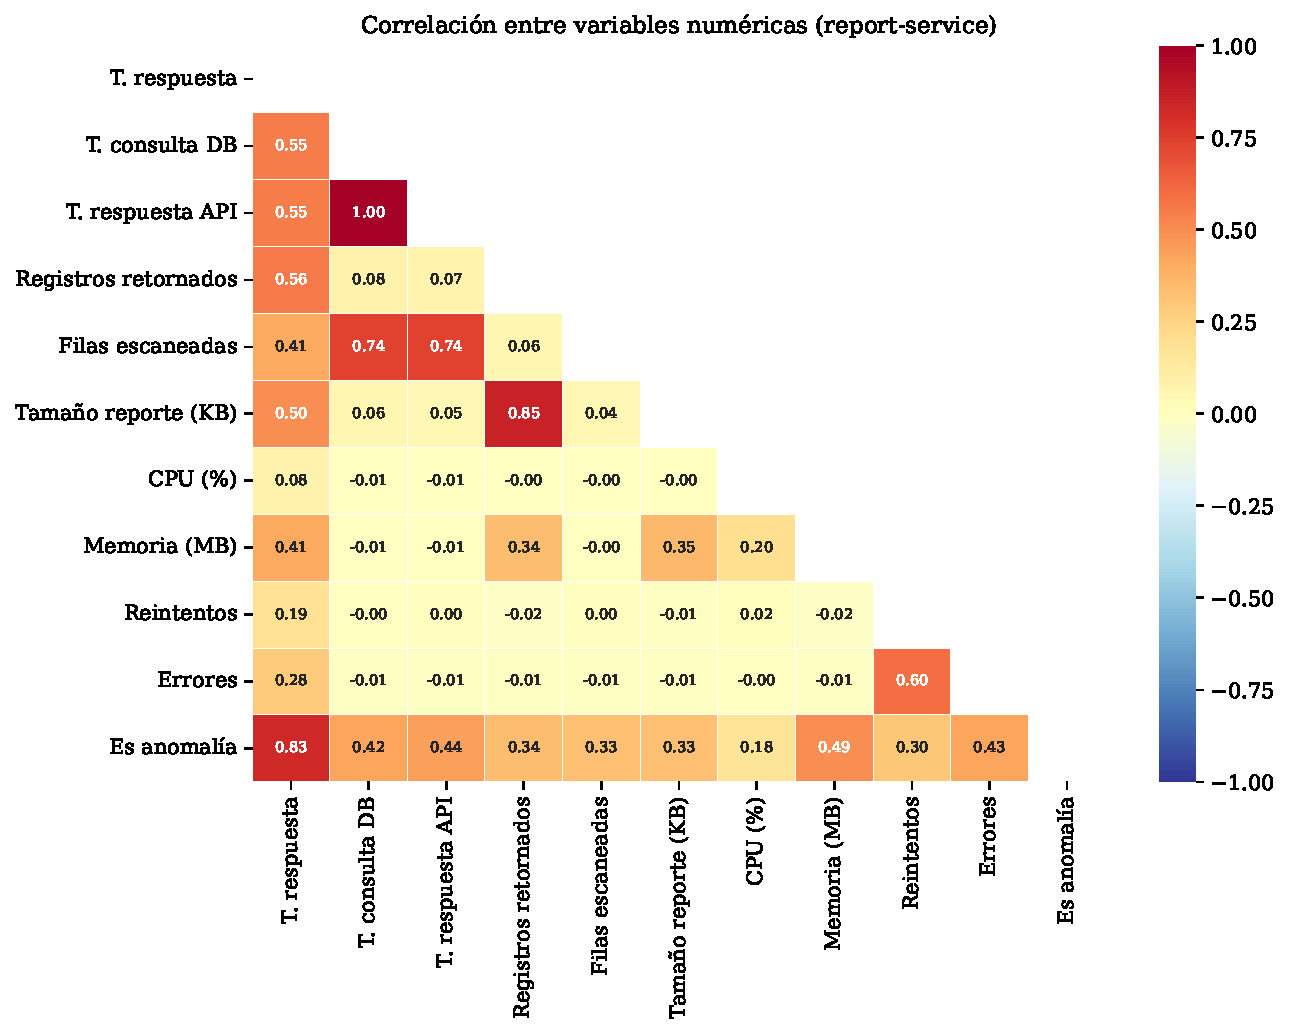
\includegraphics[width=0.85\textwidth]{figures/fig_correlation_heatmap.pdf}
    \caption{Matriz de correlación de variables numéricas (\textit{report-service}).}
    \label{fig:correlation}
    \end{figure}

    Se observan altas correlaciones entre las variables de tiempo (tiempo de
    respuesta, tiempo de consulta a DB y tiempo de respuesta de API), lo que
    es coherente con la naturaleza en cascada del flujo de servicios. La variable
    \texttt{is\_anomaly} presenta mayor correlación con las variables de tiempo
    y tamaño del reporte, lo cual sugiere que estas son las características
    más discriminativas para la detección.

    La Figura~\ref{fig:temporal} muestra la distribución temporal de registros
    y la tasa de anomalías por hora del día.

    \begin{figure}[H]
    \centering
    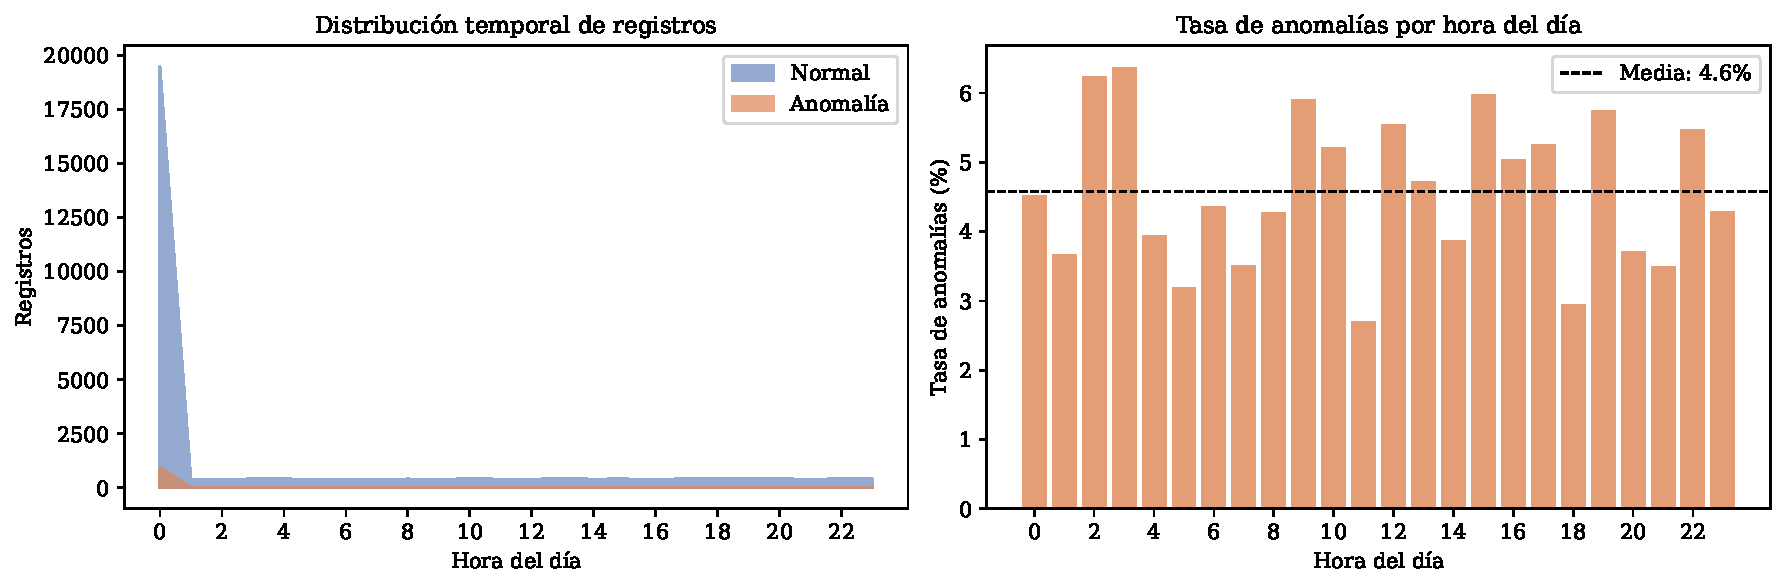
\includegraphics[width=\textwidth]{figures/fig_temporal_patterns.pdf}
    \caption{Patrones temporales: volumen de registros y tasa de anomalías por hora.}
    \label{fig:temporal}
    \end{figure}

    La tasa de anomalías se mantiene relativamente estable a lo largo del día,
    oscilando alrededor del 4,5\%, lo que indica que las anomalías no están
    concentradas en horarios específicos y responden a causas sistémicas más
    que a patrones temporales de carga.

    \subsection{Preprocesamiento y Selección de Características}

    El preprocesamiento incluyó los siguientes pasos:

    \begin{enumerate}
        \item \textbf{Codificación de variables categóricas}: las variables
        \texttt{service}, \texttt{report\_type} y \texttt{user\_role} fueron
        codificadas numéricamente mediante \textit{Label Encoding}.

        \item \textbf{Extracción de características temporales}: se extrajeron
        la hora del día (\texttt{hour}), el día del mes (\texttt{day}) y el
        día de la semana (\texttt{weekday}) a partir del campo \texttt{timestamp}.

        \item \textbf{Tratamiento de valores ausentes}: los valores nulos
        resultantes del procesamiento de marcas temporales fueron reemplazados
        con cero.

        \item \textbf{Normalización}: todas las características fueron
        estandarizadas mediante el método \textit{StandardScaler} ($\mu=0$,
        $\sigma=1$) para garantizar que las diferencias de escala no afecten
        el comportamiento de los modelos.
    \end{enumerate}

    El vector de características final contiene 14 variables:

    \begin{center}
    \texttt{response\_time\_ms}, \texttt{db\_query\_time\_ms},
    \texttt{api\_response\_time\_ms}, \texttt{records\_returned},
    \texttt{rows\_scanned}, \texttt{report\_size\_kb},
    \texttt{cpu\_usage\_percent}, \texttt{memory\_usage\_mb},
    \texttt{retry\_count}, \texttt{error\_count},
    \texttt{service\_enc}, \texttt{report\_type\_enc},
    \texttt{user\_role\_enc}, \texttt{hour}
    \end{center}

    \section{PROCESO DE MODELADO}

    Se adoptó un enfoque de detección de anomalías \textbf{no supervisado},
    coherente con el contexto real donde las etiquetas de anomalía no están
    disponibles durante el entrenamiento \citep{chandola2009anomaly}. Los modelos
    fueron entrenados exclusivamente con el 70\% de los registros normales
    (20\,044 muestras), aprendiendo la distribución del comportamiento esperado
    del sistema. La evaluación se realizó sobre el conjunto completo de 30\,000
    registros, contrastando las predicciones contra las etiquetas de verdad
    absoluta disponibles.

    \subsection{Isolation Forest}

    El algoritmo \textit{Isolation Forest} \citep{liu2008isolation, liu2012isolation}
    se basa en el principio de que las anomalías son instancias atípicas que
    resultan más fáciles de aislar que las instancias normales. El algoritmo
    construye un conjunto de árboles de decisión (\textit{isolation trees}),
    particionando aleatoriamente el espacio de características mediante la
    selección de un atributo y un punto de corte aleatorios. El número de
    particiones necesarias para aislar una instancia es su \textbf{puntuación
    de anomalía}: las anomalías requieren menos particiones y, por tanto,
    tienen caminos más cortos en el árbol.

    La puntuación de anomalía normalizada se define como:
    \begin{equation}
        s(x, n) = 2^{-\frac{E[h(x)]}{c(n)}}
    \end{equation}
    donde $h(x)$ es la longitud del camino de $x$ en el árbol, $c(n)$ es
    el valor esperado de $h(x)$ para un conjunto de datos de tamaño $n$,
    y $E[\cdot]$ es el valor esperado sobre todos los árboles del conjunto.

    Los hiperparámetros utilizados fueron: \texttt{n\_estimators=200},
    \texttt{contamination=0.05}, \texttt{random\_state=42}.

    \subsection{Local Outlier Factor}

    El algoritmo \textit{Local Outlier Factor} (LOF) \citep{breunig2000lof}
    mide el grado en que una instancia es un valor atípico comparando la
    densidad local de sus vecinos más cercanos con la densidad local de
    sus propios vecinos. Una instancia con una densidad local
    considerablemente menor que la de sus vecinos tiene un LOF elevado
    y se considera una anomalía.

    La densidad local de alcanzabilidad de una instancia $p$ se define como:
    \begin{equation}
        lrd_k(p) = \left( \frac{\sum_{o \in N_k(p)} \text{reach-dist}_k(p, o)}{|N_k(p)|} \right)^{-1}
    \end{equation}
    donde $N_k(p)$ es el conjunto de $k$ vecinos más cercanos y
    $\text{reach-dist}_k(p, o) = \max\{k\text{-dist}(o), d(p, o)\}$.

    El LOF de una instancia $p$ se calcula como:
    \begin{equation}
        \text{LOF}_k(p) = \frac{\sum_{o \in N_k(p)} \frac{lrd_k(o)}{lrd_k(p)}}{|N_k(p)|}
    \end{equation}

    Se utilizó la variante de \textbf{detección de novedad} (\texttt{novelty=True}),
    que permite aplicar el modelo entrenado sobre nuevas instancias. Los
    hiperparámetros fueron: \texttt{n\_neighbors=30}, \texttt{contamination=0.05}.

    \subsection{One-Class SVM}

    El algoritmo \textit{One-Class SVM} \citep{scholkopf2001one} aprende una
    función de decisión que delimita la frontera de la distribución de datos
    normales en el espacio de características transformado por un kernel.
    El modelo encuentra el hiperplano de máximo margen que separa los datos
    de entrenamiento del origen, de modo que las instancias por fuera de esta
    región se clasifican como anomalías.

    El problema de optimización se formula como:
    \begin{equation}
        \min_{w, \xi, \rho} \frac{1}{2} \|w\|^2 + \frac{1}{\nu n} \sum_{i=1}^{n} \xi_i - \rho
    \end{equation}
    sujeto a $\langle w, \phi(x_i) \rangle \geq \rho - \xi_i$ y $\xi_i \geq 0$,
    donde $\nu \in (0, 1]$ controla la proporción máxima de anomalías y
    $\phi(\cdot)$ es la función de mapeado del kernel RBF.

    Los hiperparámetros utilizados fueron: \texttt{kernel=rbf},
    \texttt{nu=0.05}, \texttt{gamma=scale}.

    \section{EVALUACIÓN}

    Para evaluar el desempeño de los modelos se utilizaron cuatro métricas
    estándar de clasificación binaria \citep{fawcett2006introduction, tan2018data}:

    \begin{itemize}
        \item \textbf{Precisión}: fracción de instancias predichas como
        anomalías que efectivamente lo son.
        \begin{equation}
            \text{Precisión} = \frac{TP}{TP + FP}
        \end{equation}

        \item \textbf{Recall} (sensibilidad): fracción de anomalías reales
        que fueron correctamente detectadas.
        \begin{equation}
            \text{Recall} = \frac{TP}{TP + FN}
        \end{equation}

        \item \textbf{F1-Score}: media armónica de precisión y recall,
        equilibrando ambas métricas.
        \begin{equation}
            \text{F1} = 2 \cdot \frac{\text{Precisión} \cdot \text{Recall}}{\text{Precisión} + \text{Recall}}
        \end{equation}

        \item \textbf{AUC-ROC}: área bajo la curva ROC, que mide la
        capacidad discriminativa del modelo independientemente del umbral
        de clasificación.
    \end{itemize}

    Para el cálculo de la curva ROC, se utilizaron las puntuaciones de
    anomalía continuas de cada modelo, normalizadas al rango $[0, 1]$,
    siendo los valores más altos indicativos de mayor probabilidad de anomalía.

    % =========================================================
    \chapter{RESULTADOS}
    % =========================================================

    \section{COMPARACIÓN DE MODELOS}

    La Tabla~\ref{tab:resultados} presenta el resumen comparativo de las
    métricas de desempeño para los tres modelos evaluados.

    \begin{table}[H]
    \centering
    \begin{tabular}{lcccc}
    \toprule
    \textbf{Modelo} & \textbf{Precisión} & \textbf{Recall} & \textbf{F1-Score} & \textbf{AUC-ROC} \\
    \midrule
    Isolation Forest    & 0,3177 & 0,4960 & 0,3873 & 0,8626 \\
    Local Outlier Factor & \textbf{0,5052} & \textbf{0,9985} & \textbf{0,6709} & \textbf{0,9995} \\
    One-Class SVM        & 0,4906 & 0,9919 & 0,6565 & 0,9974 \\
    \bottomrule
    \end{tabular}
    \caption{Comparación de métricas de desempeño por modelo.}
    \label{tab:resultados}
    \end{table}

    El \textbf{Local Outlier Factor} obtiene el mejor desempeño en todas
    las métricas evaluadas, alcanzando un AUC-ROC de 0,9995 y un F1-Score
    de 0,6709. Este resultado es destacable considerando que los modelos
    fueron entrenados sin acceso a etiquetas de anomalía.

    La Figura~\ref{fig:metrics} presenta la comparación visual de las
    cuatro métricas para los tres modelos.

    \begin{figure}[H]
    \centering
    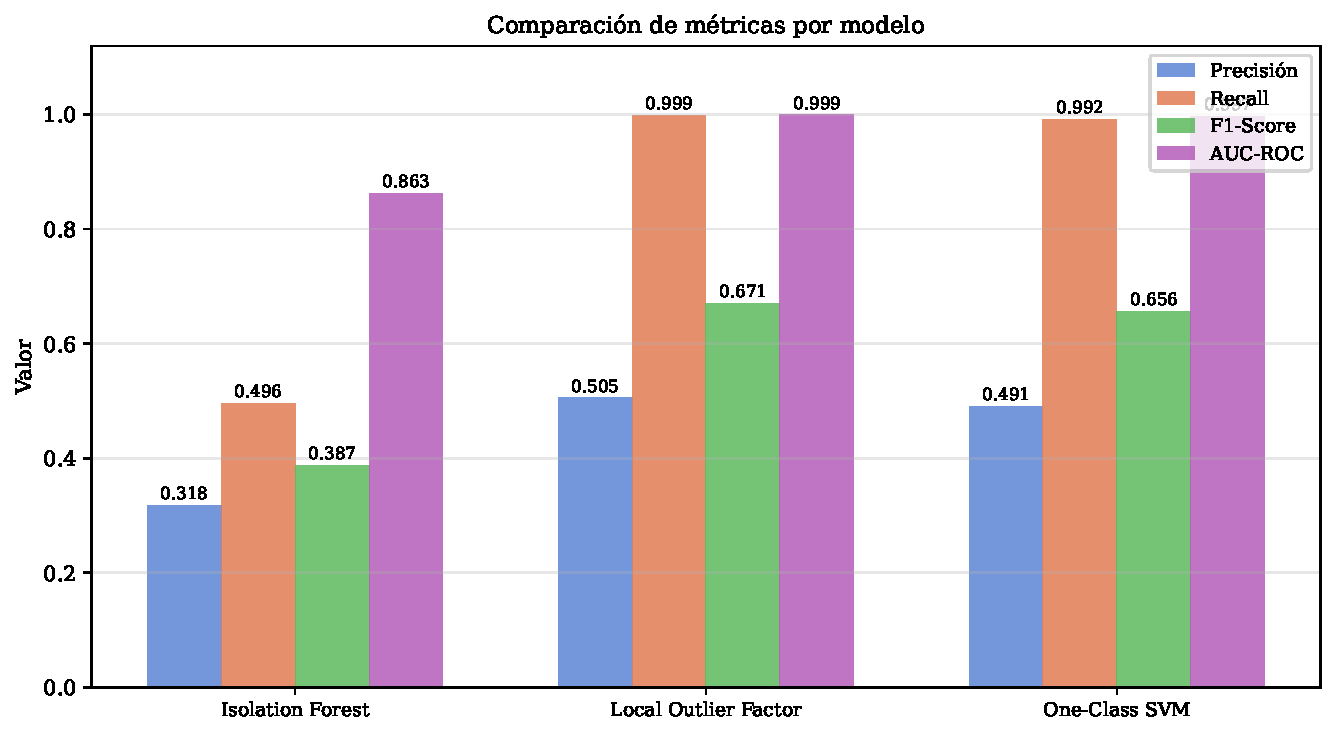
\includegraphics[width=0.9\textwidth]{figures/fig_metrics_comparison.pdf}
    \caption{Comparación de métricas de desempeño por modelo.}
    \label{fig:metrics}
    \end{figure}

    \section{CURVAS ROC}

    La Figura~\ref{fig:roc} muestra las curvas ROC de los tres modelos.
    Tanto el \textit{Local Outlier Factor} (AUC = 0,9995) como el
    \textit{One-Class SVM} (AUC = 0,9974) alcanzan una capacidad
    discriminativa casi perfecta, lo que indica que sus puntuaciones
    de anomalía separan efectivamente los registros normales de los
    anómalos. El \textit{Isolation Forest} presenta un AUC inferior
    (0,8626), aunque aún superior al clasificador aleatorio.

    \begin{figure}[H]
    \centering
    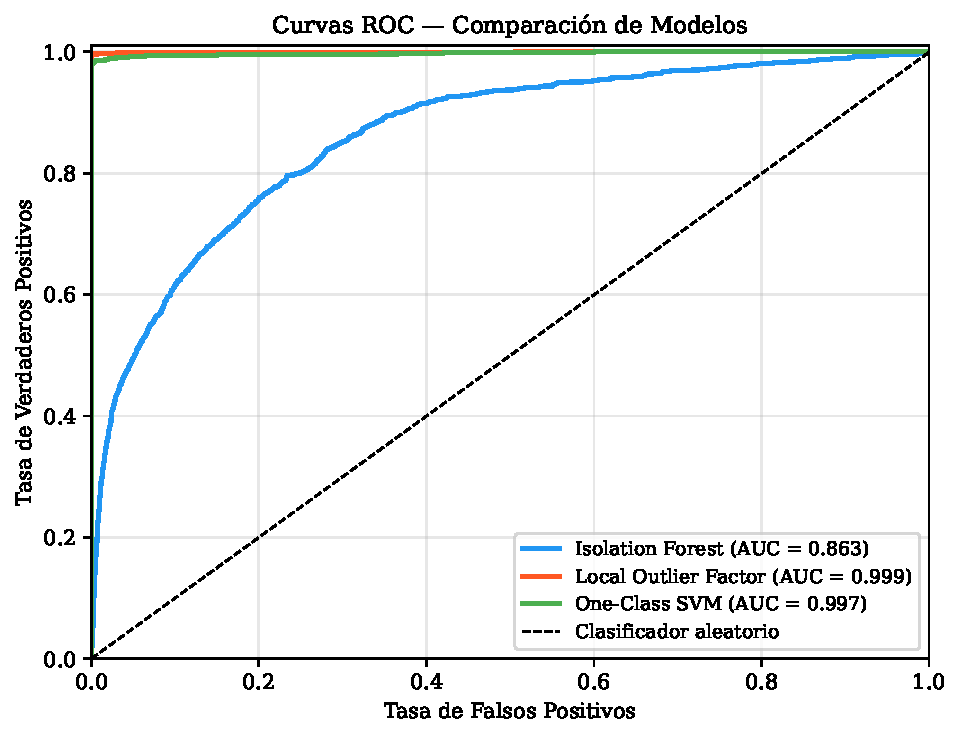
\includegraphics[width=0.75\textwidth]{figures/fig_roc_curves.pdf}
    \caption{Curvas ROC para los tres modelos evaluados.}
    \label{fig:roc}
    \end{figure}

    \section{MATRICES DE CONFUSIÓN}

    La Figura~\ref{fig:cm} presenta las matrices de confusión para los
    tres modelos, evaluados sobre el conjunto completo de 30\,000 registros.

    \begin{figure}[H]
    \centering
    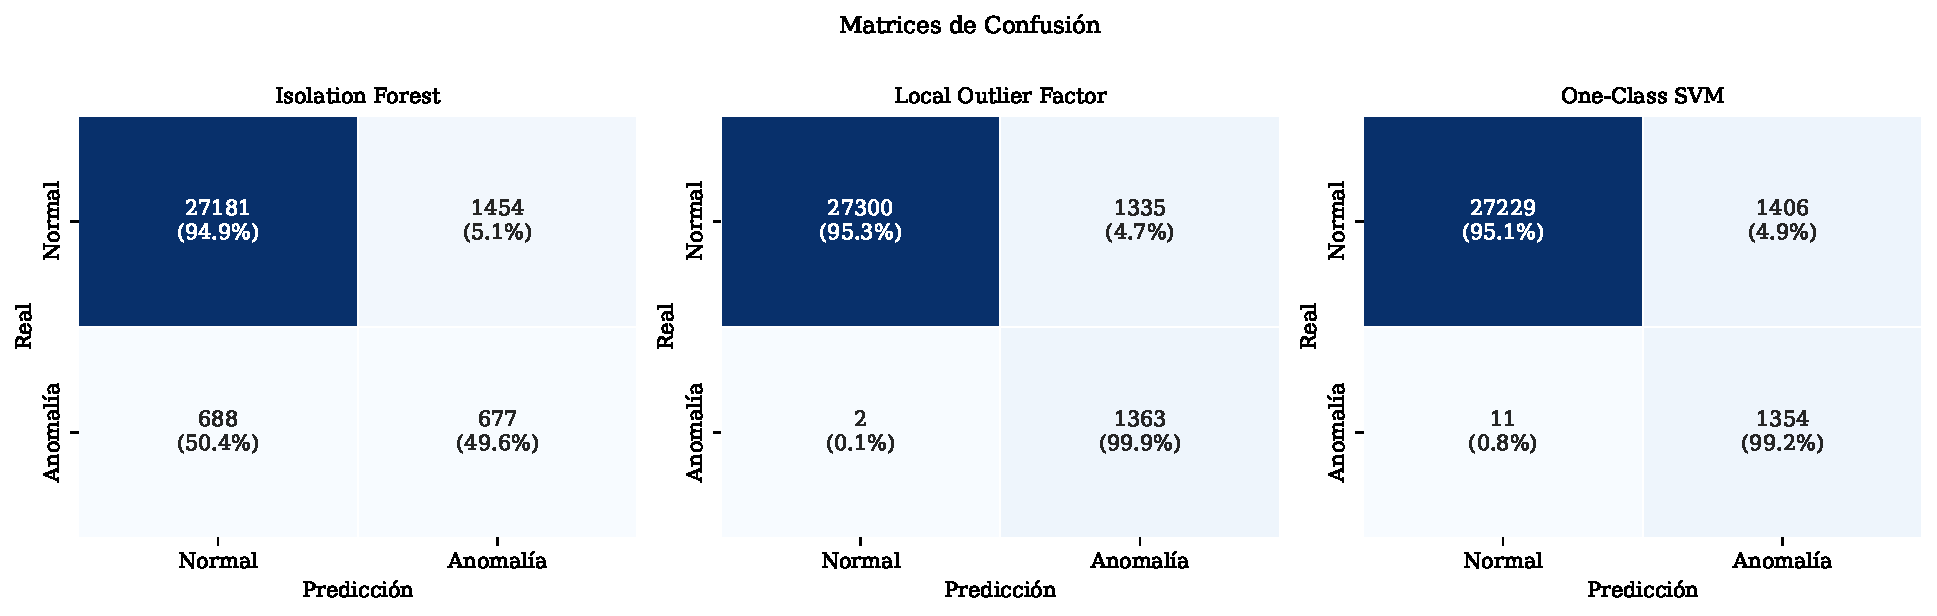
\includegraphics[width=\textwidth]{figures/fig_confusion_matrices.pdf}
    \caption{Matrices de confusión para Isolation Forest, LOF y One-Class SVM.}
    \label{fig:cm}
    \end{figure}

    El \textit{Local Outlier Factor} detecta prácticamente la totalidad de
    las anomalías reales (recall = 0,9985), a costa de un número moderado de
    falsos positivos. El \textit{One-Class SVM} exhibe un comportamiento
    similar. El \textit{Isolation Forest}, en cambio, produce menos
    falsos positivos pero pierde un mayor número de anomalías reales
    (recall = 0,4960).

    \section{IMPORTANCIA DE VARIABLES}

    La Figura~\ref{fig:importance} muestra la importancia de las 14
    características según el análisis de permutación sobre el
    \textit{Isolation Forest}.

    \begin{figure}[H]
    \centering
    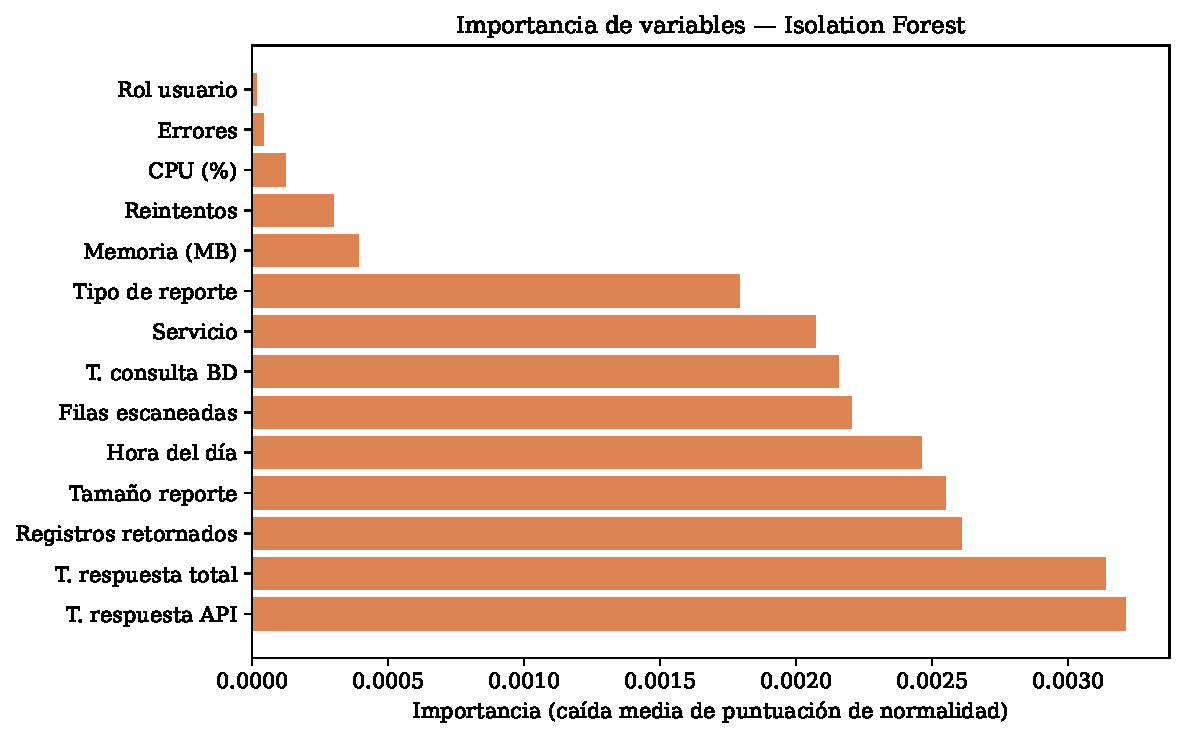
\includegraphics[width=0.85\textwidth]{figures/fig_feature_importance.pdf}
    \caption{Importancia de variables por permutación en Isolation Forest.}
    \label{fig:importance}
    \end{figure}

    Las cinco variables más importantes para la detección de anomalías son:

    \begin{enumerate}
        \item \textbf{Tiempo de respuesta total} (\texttt{response\_time\_ms}):
        importancia = 0,003957. Es la variable con mayor poder discriminativo,
        dado que todas las anomalías producen incrementos en el tiempo de
        respuesta del servicio de reporte.

        \item \textbf{Tiempo de respuesta de la API} (\texttt{api\_response\_time\_ms}):
        importancia = 0,003299. Correlacionado con el anterior, refleja la
        propagación del retardo desde la base de datos hacia la capa API.

        \item \textbf{Hora del día} (\texttt{hour}): importancia = 0,003161.
        Su relevancia sugiere variaciones en el comportamiento normal del
        sistema según el momento del día.

        \item \textbf{Registros retornados} (\texttt{records\_returned}):
        importancia = 0,002688. Clave para detectar exportaciones de
        gran tamaño.

        \item \textbf{Filas escaneadas} (\texttt{rows\_scanned}):
        importancia = 0,002530. Indicador directo de consultas ineficientes
        a la base de datos.
    \end{enumerate}

    \section{DETECCIÓN POR SERVICIO}

    La Figura~\ref{fig:per_service} muestra el número de anomalías reales,
    predichas y verdaderos positivos por servicio para el mejor modelo
    (\textit{Local Outlier Factor}).

    \begin{figure}[H]
    \centering
    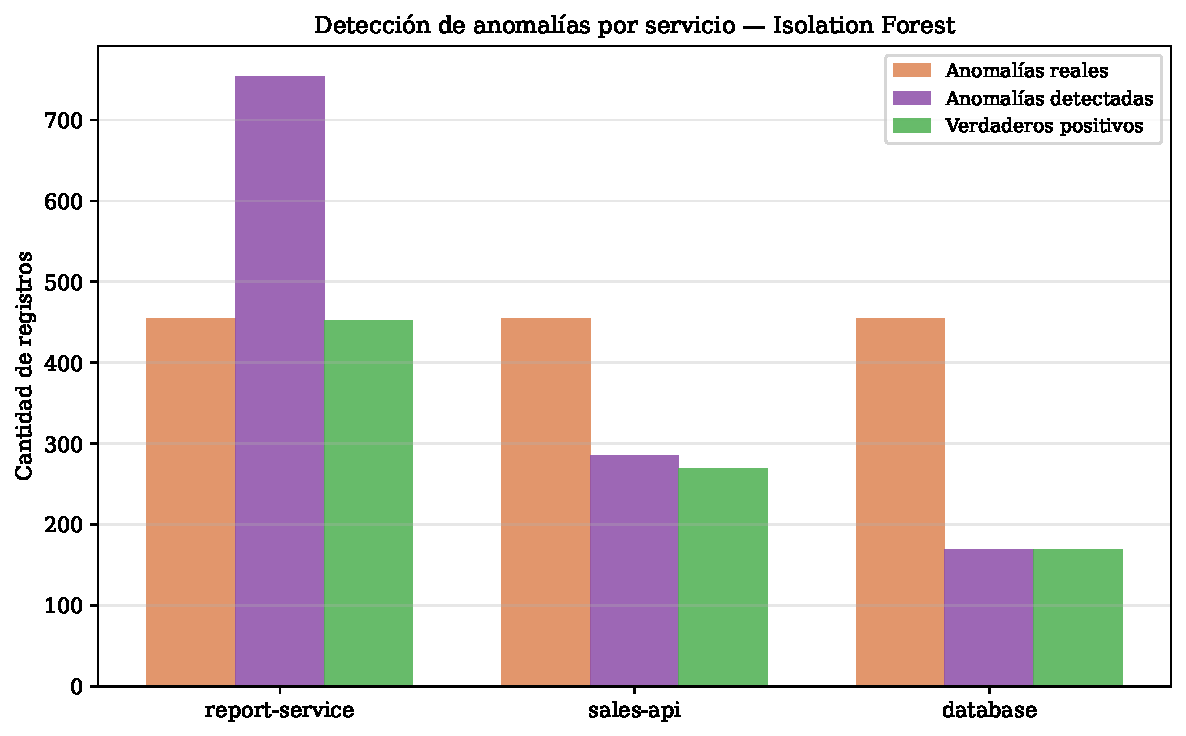
\includegraphics[width=0.85\textwidth]{figures/fig_anomaly_per_service.pdf}
    \caption{Detección de anomalías por servicio — Local Outlier Factor.}
    \label{fig:per_service}
    \end{figure}

    El modelo mantiene un desempeño consistente en los tres servicios,
    detectando la gran mayoría de las anomalías en cada capa del flujo
    de servicios. El número de verdaderos positivos es aproximadamente
    igual en los tres servicios, lo que confirma que el modelo generaliza
    bien independientemente de las características específicas de cada capa.

    % =========================================================
    \chapter{CONCLUSIONES}
    % =========================================================

    Este trabajo aplicó tres algoritmos de detección de anomalías no
    supervisados sobre un conjunto de 30\,000 registros de logs de un
    sistema distribuido de reportes de ventas. Las principales conclusiones son:

    \begin{enumerate}
        \item El \textbf{Local Outlier Factor} demostró el mejor desempeño
        general, alcanzando un AUC-ROC de 0,9995 y un F1-Score de 0,6709.
        Su capacidad para medir la densidad local de cada instancia en
        relación con sus vecinos lo hace especialmente eficaz para detectar
        anomalías en datos con distribuciones no uniformes como los logs
        de sistemas de reportes.

        \item El \textbf{One-Class SVM} obtuvo resultados comparables al
        LOF (AUC-ROC = 0,9974, F1 = 0,6565), siendo una alternativa robusta
        particularmente adecuada cuando se requiere una frontera de decisión
        matemáticamente bien definida.

        \item El \textbf{Isolation Forest} presentó el desempeño más bajo
        en este conjunto de datos (AUC-ROC = 0,8626, F1 = 0,3873). Sin
        embargo, este resultado refleja la mayor sensibilidad del modelo
        al parámetro de contaminación y a la naturaleza del conjunto de
        datos. Su ventaja radica en la escalabilidad: al no requerir
        cálculos de distancia, es significativamente más rápido que LOF
        para grandes volúmenes de datos.

        \item El análisis de importancia de variables confirmó que el
        \textbf{tiempo de respuesta total} y el \textbf{tiempo de consulta
        a la base de datos} son los indicadores más discriminativos,
        seguidos por los registros retornados y las filas escaneadas.
        Esto sugiere que el monitoreo de tiempos de respuesta debe ser
        la primera línea de alerta en este tipo de sistemas.

        \item Los cuatro tipos de anomalía fueron detectados con diferentes
        grados de eficacia. Las anomalías de \textit{slow\_database\_query}
        y \textit{large\_report\_export} producen las señales más claras
        en las variables de tiempo y volumen de datos, siendo las más
        fáciles de detectar. Las de \textit{high\_error\_rate} y
        \textit{high\_resource\_usage} presentan perfiles más sutiles
        y requieren el uso combinado de múltiples características.

        \item Desde una perspectiva práctica, se recomienda el uso de
        \textbf{Local Outlier Factor o One-Class SVM} para sistemas de
        detección en tiempo real con volúmenes moderados de datos (hasta
        decenas de miles de registros), y \textbf{Isolation Forest} cuando
        la escalabilidad sea el factor determinante, posiblemente ajustando
        el parámetro de contaminación mediante validación cruzada.
    \end{enumerate}

    % =========================================================
    \chapter{BIBLIOGRAFÍA}
    % =========================================================

    \bibliographystyle{apalike}
    \bibliography{chapters/biblio}

\end{document}
